\subsubsection{Simulinks PID Clamping Anti-Windup Problematik}
\label{sec:Description_SimulinkPID_ClampingLogic_Problem}
In Simulink wird die Clamping Anti-Windup Methode etwas UNDers umgesetzt als in dieser Arbeit beschrieben.
In der Dokumentation für den PID-Regler Block \cite{matlabPIDController} wird die Clamping Logik wie folgt definiert:
% zitat:
\begin{quote}
    \label{quote:SimulinkPID_Clamping}
    \textit{\textbf{clamping}}\\
    \textit{Integration stops when the sum of the block components exceeds the output limits UND the integrator output UND block input have the same sign. 
    Integration resumes when the sum of the block components exceeds the output limits UND the integrator output UND block input have opposite sign. 
    Clamping is sometimes referred to as conditional integration.\\
    Clamping can be useful for plants with relatively small dead times, but can yield a poor transient response for large dead times.}
\end{quote}

Wie sich herausgestellt hat, ist die Tatsächliche Implementierung nicht so wie in der Dokumentation beschrieben.
Bei bestimmten $Kp$, $Ki$ und $Kd$ Kombinationen kann es teilweise zu unerwünschtem Verhalten am Ausgang des PID-Reglers kommen.

\horizontalLine
\minipagedOrBelowEachOther{
    Die~\ref{fig:ResponseMatlabPID_clampingProblem} zeigt das Verhalten des PID-Reglers beim ausschalten des Motors. 
    In orange ist der Regler-Ausgang $u$ dargestellt, welcher die Spannung am Motor repräsentiert.
    In blau ist die Drehgeschwindigkeit $y$ des Motors dargestellt.
    Beim ausschalten des Motors (Referenz auf 0 setzen) sollte der Regler-Ausgang $u$ auf 0 gehen und bleiben. 
    Es ist jedoch zu erkennen, dass der Regler plötzlich beginnt kleine Rippel zu erzeugen. 
    Diese Rippel führen dazu, dass der Motor immer wieder kurz anläuft und wieder stoppt, was zu einem unerwünschten Verhalten führt.
}
{
    \begin{figure}[H]
        \centering
            \includegraphics[width=0.4\linewidth]{images/ResponseMatlabPID_clampingProblem.pdf}
            \caption{
                \centering
                Motor ausschalten mit Simulink PID-Regler und Clamping Anti-Windup \\
                $Kp=5$, $Ki=35$, $Kd=0$
            }
        \label{fig:ResponseMatlabPID_clampingProblem}
    \end{figure}
}

\paragraph{Clamping Logik}
\begin{figure}[H]
    \centering
    \includegraphics[width=0.98\linewidth]{images/SimulinkPID_clampingLogic.pdf}
    \caption{Clamping Logik im Simulink PID-Regler \cite{matlabPIDController}}
    \label{fig:SimulinkPID_clampingLogic}
\end{figure}
Die Eingänge dieses Blockes sind:
\begin{itemize}
    \item $preSat$: Welches dem Signal $u_{\mathrm{preSat}}$ aus der~\fullref{fig:ErweiterterPID} entspricht.
    \item $Upper Limit$: Ist das obere Sättigungs-Limit am Ausgang des PID-Reglers. $Upper Limit = 10$
    \item $Lower Limit$: Ist das untere Sättigungs-Limit am Ausgang des PID-Reglers. $Lower Limit = 0$
    \item $preInt$: Ist das Signal vor dem Integrator, also $e \cdot Ki$.
\end{itemize}

Der Ausgang links mit dem Namen \textit{1} ist der effektive Integrator Eingang nach der Clamping Logik.


\newpage
\subparagraph{Logikbeschreibung}
\noindent
\\
\minipagedOrBelowEachOther{
    Die Eingangssignale $preSat$, $Upper Limit$ und $Lower Limit$ werden im Block \textit{Dead Zone} verarbeitet.\\


    Der Ausgang $Clamping\_zero$ (Signal-Name) der Dead Zone ist negativ, wenn sich der PID-Regler in der negativen Sättigung befindet.
    Er ist positiv, wenn sich der PID-Regler in der positiven Sättigung befindet.
    Wenn $Clamping\_zero \neq 0$, dann ist der erste Eingang am $UND-Gatter$ aktiv.
    Der zweite Eingang am $UND-Gatter$ ist aktiv, wenn $preInt$ und $Clamping\_zero$ das gleiche Vorzeichen haben.
    Wenn der Ausgang am $UND-Gatter$ aktiv ist, wird der Integrator Eingang auf 0 gesetzt.\\
}
{
    \begin{figure}[H]
        \centering
        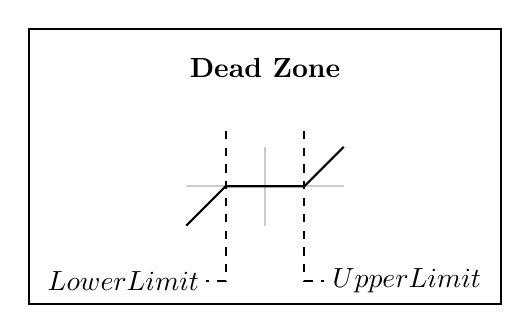
\begin{tikzpicture}[thick]
            \definecolor{lightGrayColor}{rgb}{0.8,0.8,0.8};
            % Block rectangle
            \draw (0,0) rectangle (6,3.5);
            % Title "Dead Zone"
            \node at (3,3) {\textbf{Dead Zone}};
            % Daw axis
            \draw[color=lightGrayColor] (2, 1.5) -- (4, 1.5); % Horizontal line
            \draw[color=lightGrayColor] (3, 1.0) -- (3, 2.0); % Vertical line
            % Characteristic curve inside the block
            \draw (2,1) -- (2.5,1.5) -- (3.5,1.5) -- (4,2);
            % Vertical lines indicating the dead zone region
            \draw[dashed] (2.5,2.2) -- (2.5,0.3) -- (2.25,0.3);
            \draw[dashed] (3.5,2.2) -- (3.5,0.3) -- (3.75,0.3);
            
            % Labels
            \node[] at (1.2,0.3) {$Lower Limit$};
            \node[] at (4.8,0.3) {$Upper Limit$};
        \end{tikzpicture}
        \caption{Dead Zone Charakteristik}
        \label{fig:SimulinkPID_clampingLogic_deadZone}
    \end{figure} 
}


\horizontalLine
\subparagraph{Problematik bei dieser Logik}
\noindent
\\
Das Vergleichen des Vorzeichens ist grundsätzlich richtig, aber $preSat$ ist nicht das richtige Signal dafür.
Was in~\ref{fig:ResponseMatlabPID_clampingProblem} passiert ist folgendes:
\begin{itemize}
    \item Zeitpunkt wo $r$ auf 0 gesetzt wird:
    \begin{itemize} 
        \item Der Integrator hat einen Wert von ca. 2 gespeichert.
        \item Der Proportionalteil schlägt in den negativen Bereich mit einem Wert von $Ki \cdot e=5 \cdot -2=-10$ aus.
        \item Somit ist $preSat = -10 + 2 + 0 = -8$.
        \item Da $preSat < Lower Limit$ folgt $\rightarrow$ $Clamping\_zero < 0$.
        \item $PreInt = Ki \cdot e = 35 \cdot -2 = -70$
        \item $sgn(PreInt) = sgn(Clamping\_zero)$ $\rightarrow$ Integrator Eingang = 0
        \item Der Integrator bleibt auf 2 stehen.
    \end{itemize}
    \item Der Ausgang des PID-Reglers ist in der unteren Sättigung bei 0, deshalb dreht der Motor nur noch aus.
    \item Sobald der Term $Kp \cdot e + Ui > 0$ wird, befindet sich das Signal $preSat$ nicht mehr im gesättigten Bereich.
    Was dann passiert ist folgendes:
    \begin{itemize}
        \item $Kp \cdot e + Ui = 0$ $\rightarrow$ $e = \frac{-Ui}{Kp} = \frac{-2}{5} = -0.4$    
        \item $Clamping\_zero = 0$ $\rightarrow$ Der erste Eingang am $UND-Gatter$ ist nicht mehr aktiv.
        \item Da der erste Eingang am $UND-Gatter$ nicht mehr aktiv ist, wird der Integrator Eingang wieder auf $preInt$ gesetzt.
        \item Der Integrator beginnt nun wieder abzuintegrieren.
    \end{itemize}
    \item Der Integrator integriert schneller ab als der Motor abbremst, was was dazu führt, dass 
    $Kp \cdot e + Ui < 0$ wird und der PID-Regler wieder in die negative Sättigung geht.
    \item Dadurch wird $Clamping\_zero$ wieder negativ und der Integrator Eingang wieder auf 0 gesetzt.
    \item Dieses Verhalten wiederholt sich, was zu den Rippeln am Ausgang des PID-Reglers führt.
\end{itemize}
Das Verhalten ist unten in \ref{fig:SimulinkPID_clampingLogicPlot} dargestellt.
\newpage



\begin{figure}[H]
    \centering
        \includegraphics[width=1.4\linewidth, angle=90]{images/SimulinkPID_clampingLogicPlot.png}
        \caption{Interne Signale des PID-Reglers während der Entstehung der Rippel}
    \label{fig:SimulinkPID_clampingLogicPlot}
\end{figure}
\newpage

\subparagraph{Lösung des Problems}
\noindent
\\
\infoBlock{Die folgende Implementierung ist in der C++ PID-Implementierung umgesetzt.}

Wenn man die Implementierung so umsetzt, wie sie in der Dokumentation \ref{quote:SimulinkPID_Clamping} beschrieben ist,
dann funktioniert die Clamping Logik wie erwartet.


\begin{figure}[H]
    \centering
    \includegraphics[width=0.98\linewidth]{images/SimulinkPID_clampingLogic_edited.pdf}
    \caption{Verbesserte clamping Logik im Simulink PID-Regler}
    \label{fig:SimulinkPID_clampingLogic_edited}
\end{figure}


\horizontalLine
\minipagedOrBelowEachOther{
    Wie man in \ref{fig:ResponseMatlabPID_clampingProblem_solved} sehen kann, sind die Rippel am Ausgang des PID-Reglers 
    verschwunden. Der PID-Ausgang (orange) bleibt auf 0, wie erwartet.
    Leider lässt sich dieser Fix nicht in den Simulink PID-Regler Block integrieren, deshalb kommt dieser Effekt dennoch an einigen 
    Stellen der Dokumentation vor.
}{
    \begin{figure}[H]
        \centering
        \includegraphics[width=0.3\linewidth]{images/ResponseMatlabPID_clampingProblem_solved.pdf}
        \caption{
            \centering
            Motor ausschalten mit Simulink PID-Regler und verbesserter Clamping Anti-Windup \\
            $Kp=5$, $Ki=35$, $Kd=0$
        }
        \label{fig:ResponseMatlabPID_clampingProblem_solved}
    \end{figure}
}
